\documentclass{article}
\usepackage{graphics,tikz,tkz-graph}
\usepackage[first=0,last=8]{lcg}
\usetikzlibrary{shapes}
\tikzset{EdgeStyle/.append style = {->, bend left}}
\begin{document}
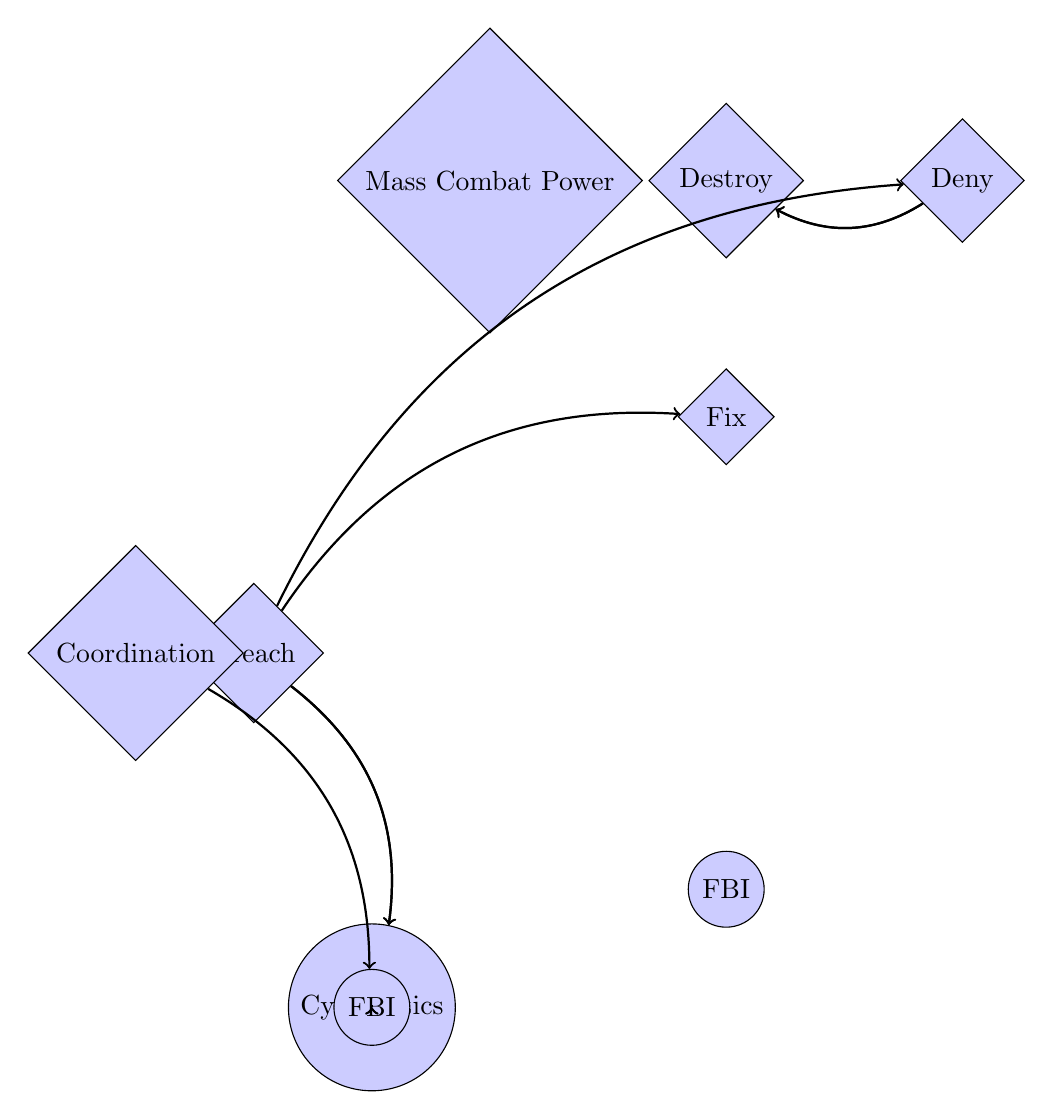
\begin{tikzpicture}
	\tikzstyle{blank} = [inner sep=0, minimum size=0]

%	\foreach \x in {0,...,8} {
%		\foreach \y in {0,...,8} {
%			\node (a\x\y) at (\x, \y) {};
%		}
%	}

	\def\milword{{"Intelligence", "Mission Command", "DOTMLPF", "Strategic Deterence", "Cybernetics", "JECC", "FBI", "UCP",
			"STRATCOM", "Warfighter", "BCT", "Operational Art"}}
	\def\milverb{{"Fix", "Disrupt", "Penetrate", "Isolate", "Interdict", "Breach", "Suppress", "Destroy",
			"Planing", "Coordination", "Mass Combat Power", "Deny"}}
	\foreach \x in {0,...,8} {
		\pgfmathrandominteger{\a}{0}{8}
		\pgfmathrandominteger{\b}{0}{8}
		\pgfmathrandominteger{\c}{0}{5}
		\pgfmathrandominteger{\d}{0}{11}
		\ifthenelse{\c<2}{
			\node[draw,diamond, fill=blue!20] (a\x) at (1.5*\a,1.5*\b) {\pgfmathparse{\milverb[\d]}\pgfmathresult};
		} {
			\node[draw,circle, fill=blue!20] (a\x) at (1.5*\a,1.5*\b) {\pgfmathparse{\milword[\d]}\pgfmathresult};
		}
	}

	\foreach \x in {0,...,8} {
		\pgfmathrandominteger{\a}{0}{8}
		\pgfmathrandominteger{\b}{0}{8}
		\ifthenelse{\a = \b} {
			\Loop[dist=2cm, dir=SO](a\x.east)
		} {
			\Edge(a\a)(a\b)
		}
	}

%	\node[draw, diamond, fill=blue!20] (0) {FLASID};
%	\node[blank, below of=0] (0a) {};
%	\node[draw, circle,fill=blue!20, below of=0a] (1) {DSCA};
%	\node[blank, right of=1] (1a) {};
%	\node[draw, circle,fill=red!20, right of=1a] (2) {OCO};
%	\node[blank, below of=2] (2a) {};
%	\node[draw, rectangle,fill=green!20, below of=2a] (3) {DOTMLPF};
%	\node[blank, right of=3] (3a) {};
%	\node[draw, rectangle,rounded corners=0.8ex, right of=3a] (4) {ULO};
%
%	\draw[thick,->] (0) to (1);
%	\Edge(1)(2)
%	\draw[thick,->] (2) to (3);
%	\Edge(3)(4)
%	\Loop[dist = 2cm, dir = SO](4.east)

\end{tikzpicture}
\end{document}
